\documentclass[11pt]{article}
\usepackage[a4paper,margin=2.2cm]{geometry}
\usepackage[T1]{fontenc}
\usepackage{amsmath,amssymb}
\usepackage{graphicx}
\usepackage{booktabs}
\usepackage{tabularx}
\usepackage{array}
\usepackage{float}
\usepackage{caption}
\usepackage{xcolor}
\usepackage{enumitem}
\usepackage{tikz}
\usetikzlibrary{positioning,arrows.meta,fit,calc}
\usepackage[colorlinks=true,linkcolor=blue!50!black,urlcolor=blue!60!black]{hyperref}

\captionsetup{font=small,labelfont=bf}
\setlist{itemsep=2pt,topsep=3pt}
\newcolumntype{Y}{>{\raggedright\arraybackslash}X}

% ---------------------------------------------------------------- fill these in
\newcommand{\studentname}{}
\newcommand{\rollnumber}{25280069}
% replace the whole definition with e.g. \newcommand{\githuburl}{\url{https://github.com/you/DL4STG-PA2}}
\newcommand{\githuburl}{\url{https://github.com/hassnainalimurtaza/AI651-PA2}}
\newcommand{\fillin}[1]{\textcolor{red}{\textbf{[FILL IN: #1]}}}
% ------------------------------------------------------------------------------

\newcommand{\q}[1]{\par\medskip\noindent\textbf{#1}\quad}
\newcommand{\gif}[1]{\texttt{\detokenize{#1}}}

\title{AI651 -- Deep Learning for Space, Time and Graphs\\ Programming Assignment 2}
\author{Roll number: \rollnumber}
\date{Fall 2026}

\begin{document}
\maketitle

\begin{center}
\fbox{\parbox{0.9\linewidth}{\centering
\textbf{Code repository (public):} \githuburl\\[2pt]
Question 2 code: \texttt{Question2/} (five Kaggle notebooks and \texttt{q2lib.py});
GIFs: \texttt{Question2/outputs/*/gifs/}.\\
All timings: NVIDIA Tesla T4 (Kaggle), PyTorch 2.11.}}
\end{center}

\tableofcontents
\newpage

% =====================================================================================
\section*{Question 1 -- River Forecasting Proposal}
\renewcommand{\thetable}{Q1.\arabic{table}}\renewcommand{\thefigure}{Q1.\arabic{figure}}
\addcontentsline{toc}{section}{Question 1 -- River Forecasting Proposal}
% =====================================================================================

\textbf{Proposed system in one sentence.} A \emph{directed river-graph forecaster}:
\begin{itemize}
  \item each station's history is encoded by a causal temporal convolution;
  \item information is passed \emph{downstream only}, along the river's edges, through \emph{lag attention}. Lag attention learns, from the current river state, how many 10-minute steps ago the upstream reading that matters was taken, so travel times are allowed to vary;
  \item a direct multi-horizon head issues \emph{quantile} forecasts of the water level at S1--S4 for $t{+}10,\dots,t{+}60$ minutes.
\end{itemize}

\subsection*{1. Architecture diagram}
\addcontentsline{toc}{subsection}{1. Architecture diagram}

\begin{figure}[H]
\centering
\resizebox{\linewidth}{!}{%
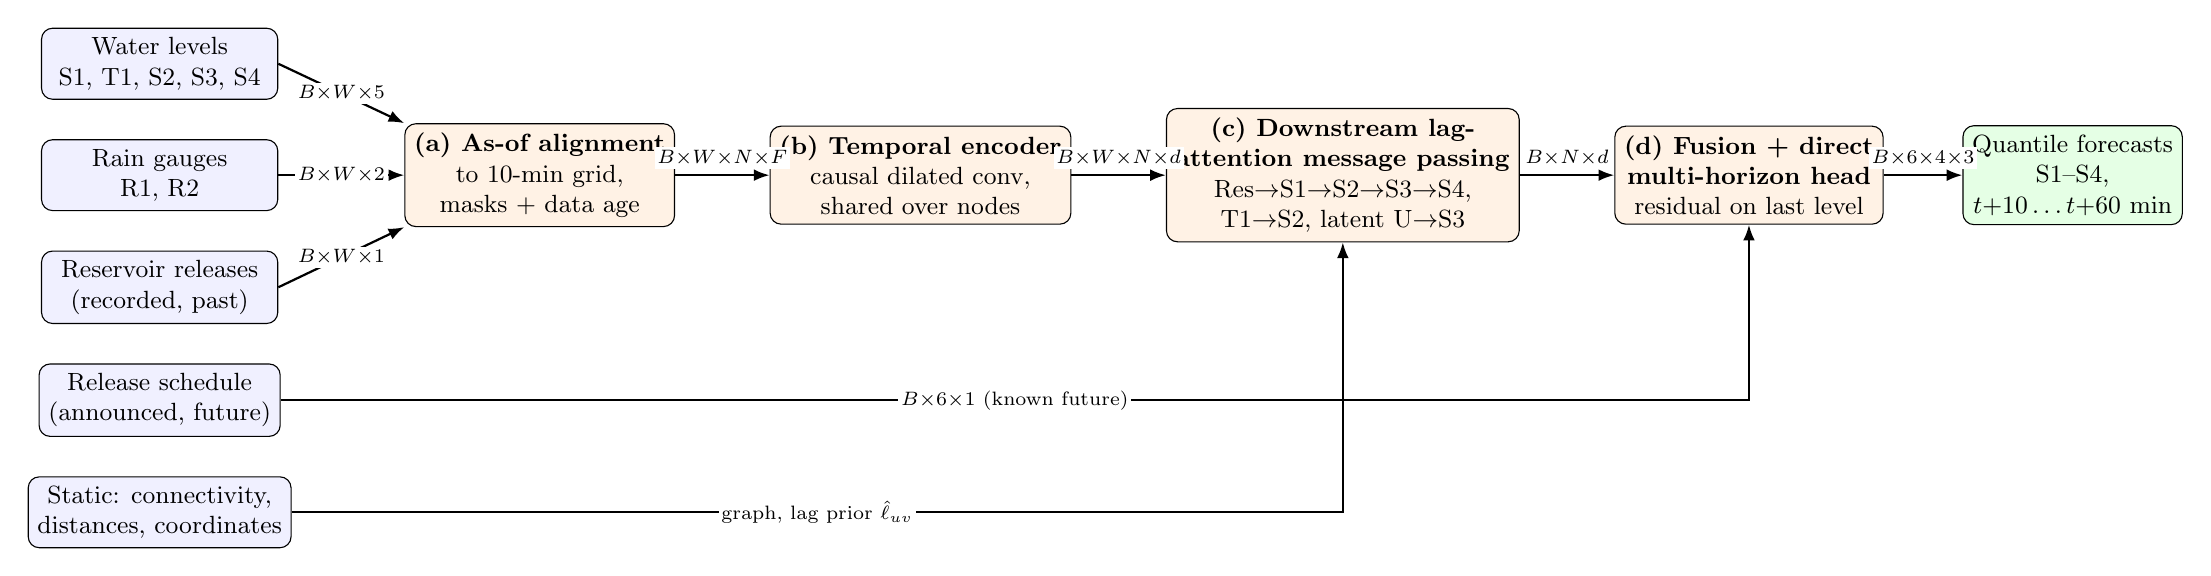
\begin{tikzpicture}[
  font=\small,
  src/.style={draw,rounded corners,fill=blue!6,align=center,minimum width=3.0cm,minimum height=0.9cm},
  blk/.style={draw,rounded corners,fill=orange!10,align=center,minimum height=0.9cm},
  outbox/.style={draw,rounded corners,fill=green!10,align=center,minimum height=0.9cm},
  arr/.style={-{Latex[length=2mm]},thick},
  lab/.style={font=\scriptsize,midway,fill=white,inner sep=1pt}]
\node[src] (lev) {Water levels\\S1, T1, S2, S3, S4};
\node[src,below=0.5cm of lev] (rain) {Rain gauges\\R1, R2};
\node[src,below=0.5cm of rain] (resp) {Reservoir releases\\(recorded, past)};
\node[src,below=0.5cm of resp] (resf) {Release schedule\\(announced, future)};
\node[src,below=0.5cm of resf] (stat) {Static: connectivity,\\distances, coordinates};
\node[blk,right=1.6cm of rain,minimum width=3.4cm] (align) {\textbf{(a) As-of alignment}\\to 10-min grid,\\masks + data age};
\node[blk,right=1.2cm of align,minimum width=3.3cm] (tenc) {\textbf{(b) Temporal encoder}\\causal dilated conv,\\shared over nodes};
\node[blk,right=1.2cm of tenc,minimum width=3.6cm] (graph) {\textbf{(c) Downstream lag-}\\\textbf{attention message passing}\\Res$\to$S1$\to$S2$\to$S3$\to$S4,\\T1$\to$S2, latent U$\to$S3};
\node[blk,right=1.2cm of graph,minimum width=3.1cm] (head) {\textbf{(d) Fusion + direct}\\\textbf{multi-horizon head}\\residual on last level};
\node[outbox,right=1.0cm of head,minimum width=2.6cm] (y) {Quantile forecasts\\S1--S4,\\$t{+}10\ldots t{+}60$ min};
\draw[arr] (lev.east) -- node[lab]{$B{\times}W{\times}5$} (align.north west);
\draw[arr] (rain.east) -- node[lab]{$B{\times}W{\times}2$} (align.west);
\draw[arr] (resp.east) -- node[lab]{$B{\times}W{\times}1$} (align.south west);
\draw[arr] (align) -- node[lab,above=2pt]{$B{\times}W{\times}N{\times}F$} (tenc);
\draw[arr] (tenc) -- node[lab,above=2pt]{$B{\times}W{\times}N{\times}d$} (graph);
\draw[arr] (graph) -- node[lab,above=2pt]{$B{\times}N{\times}d$} (head);
\draw[arr] (head) -- node[lab,above=2pt]{$B{\times}6{\times}4{\times}3$} (y);
\draw[arr] (resf.east) -| node[lab,pos=0.25]{$B{\times}6{\times}1$ (known future)} (head.south);
\draw[arr] (stat.east) -| node[lab,pos=0.25]{graph, lag prior $\hat\ell_{uv}$} (graph.south);
\end{tikzpicture}}
\caption{Architecture. $B$ = batch (number of issuance times), $W=144$ ten-minute steps (24 h of history), $N=6$ graph nodes (S1, T1, S2, S3, S4 and a latent node U for the unmonitored tributary; U has no observations), $F$ = input features per node, $d=64$ hidden width.
The output is $B\times6\times4\times3$: 6 horizons $\times$ 4 stations $\times$ quantiles $\{0.1,0.5,0.9\}$.
Alignment: all sources are resampled as of their \emph{arrival} time onto the same 10-minute grid ending at issuance time $t$. Rain is projected onto river nodes by a learned $2\to N$ map initialised with inverse-distance weights. The future schedule is a known covariate added at the head, per horizon.}
\label{fig:q1arch}
\end{figure}

\noindent The river graph used in block (c), with edges pointing downstream:

\begin{center}
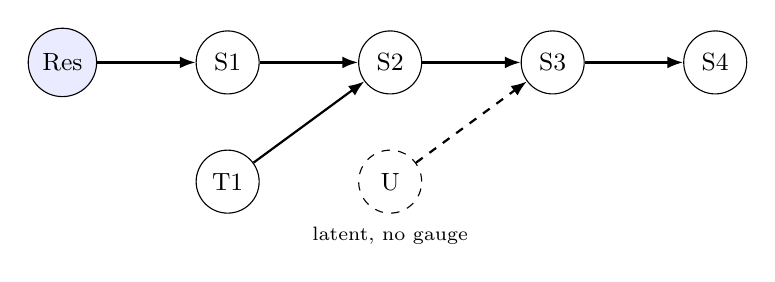
\begin{tikzpicture}[node distance=1.25cm,st/.style={circle,draw,minimum size=0.8cm,font=\small},
  arr/.style={-{Latex[length=2mm]},thick}]
\node[st,fill=blue!8] (Res) {Res};
\node[st,right=of Res] (S1) {S1};
\node[st,below=0.7cm of S1] (T1) {T1};
\node[st,right=of S1] (S2) {S2};
\node[st,dashed,below=0.7cm of S2] (U) {U};
\node[st,right=of S2] (S3) {S3};
\node[st,right=of S3] (S4) {S4};
\draw[arr] (Res)--(S1); \draw[arr] (S1)--(S2); \draw[arr] (T1)--(S2);
\draw[arr] (S2)--(S3); \draw[arr,dashed] (U)--(S3); \draw[arr] (S3)--(S4);
\node[font=\scriptsize,below=0.05cm of U] {latent, no gauge};
\end{tikzpicture}
\end{center}

\subsection*{2. Assumptions}
\addcontentsline{toc}{subsection}{2. Assumptions}

\textbf{Supplied facts (not assumptions):}
\begin{itemize}
  \item 10-minute levels at S1--S4 and T1, and timestamped rainfall at R1 and R2;
  \item recorded releases, and future schedules announced before issuance with announcement and effective times;
  \item station locations, connectivity and distances;
  \item an unmonitored tributary joining between S2 and S3;
  \item no future rainfall or future levels at issuance;
  \item precise travel times not supplied.
\end{itemize}

\begin{enumerate}[label=\textbf{A\arabic*}]
\item \textbf{The longest relevant travel time is under 12 hours.} This covers the Reservoir$\to$S4 chain plus the 1-hour horizon. \emph{Why reasonable:} the stations are a few km apart on a mountain river. \emph{Effect:} the history window is $W=144$ steps (24 h, a 2$\times$ margin), and the temporal encoder's receptive field must cover it.
\item \textbf{Water only flows downstream.} Backwater effects from S4 up to S3 are negligible. \emph{Effect:} graph edges point downstream only, so a forecast can never use information that travels upstream.
\item \textbf{Travel time varies smoothly with flow.} Higher water travels faster. \emph{Effect:} lag attention is conditioned on the current upstream level instead of using a fixed lag.
\item \textbf{The rain gauges represent their sub-catchments.} R1 mainly informs the upper reach (S1/S2 and T1); R2 mainly informs the reach of the unmonitored tributary (S3/S4). \emph{Effect:} rain is mapped onto nodes with weights that start at inverse-distance values and are then learned.
\item \textbf{Reporting delays are mostly under 30 minutes.} Records carry an arrival time, or one can be logged. \emph{Effect:} inputs are joined \emph{as of arrival}; anything later counts as missing at issuance.
\item \textbf{Measurement quality.} Level sensors have small noise and occasional flat-lines or spikes, which are filtered by range and rate-of-change checks before use. \emph{Effect:} implausible values are masked, not imputed silently.
\item \textbf{Record length.} At least 2--3 years of data exist, including several high-flow events. \emph{Effect:} a compact learned model (about $2\times10^5$ parameters) is trainable. We split the data by contiguous time blocks to avoid leakage.
\item \textbf{The datum stays the same.} Each station's zero level does not change; rating changes are rare and announced. \emph{Effect:} per-station normalisation (mean and standard deviation from the training period) is valid.
\item \textbf{Announced schedules are usually followed.} Deviations are possible and are learned from the historical announced-vs-actual record. \emph{Effect:} the schedule is a known future covariate, trusted only as much as history justifies.
\item \textbf{The unmonitored tributary responds mainly to rain near R2.} \emph{Effect:} it is modelled as a latent node U whose state is driven by R2 rainfall and learned from the S3 residual.
\end{enumerate}

\subsection*{3. Forecasting task and data specification}
\addcontentsline{toc}{subsection}{3. Forecasting task and data specification}

\begin{itemize}
\item \textbf{Issuance} happens every 10 minutes at time $t$, a multiple of 10 minutes, Coordinated Universal Time (UTC).
\item \textbf{History window:} $t-143,\dots,t$ in 10-minute steps (24 h).
\item \textbf{Horizon:} $h=1,\dots,6$, that is $t{+}10$ to $t{+}60$ minutes.
\item \textbf{Outputs:} the levels at S1--S4. T1 is used only as an input.
\end{itemize}

\begin{table}[H]
\centering\small
\caption{Inputs and outputs for one forecast. $B$ = batch (independent issuance times). Steps are 10 minutes.}
\label{tab:q1io}
\begin{tabularx}{\linewidth}{@{}l l Y Y@{}}
\toprule
Tensor & Shape & Axes & Time coverage / alignment\\
\midrule
Levels $\mathbf{Y}$ & $B\times144\times5$ & batch, step, station (S1,T1,S2,S3,S4) & $t{-}143..t$; latest valid reading at or before each step end that \emph{arrived} by $t$\\
Level mask, age & $B\times144\times5\times2$ & same; mask$\in\{0,1\}$, minutes since last valid reading & as above\\
Rainfall $\mathbf{P}$ & $B\times144\times2$ & batch, step, gauge (R1,R2) & 10-minute accumulation in $(\tau{-}10,\tau]$; mask if missing\\
Past releases $\mathbf{Q}$ & $B\times144\times1$ & batch, step & recorded mean release per step\\
Release schedule $\mathbf{S}$ & $B\times6\times2$ & batch, horizon, (scheduled release, $\mathbb{1}$[schedule exists]) & $t{+}1..t{+}6$; latest version \emph{announced} before $t$, as a step function of effective times\\
Calendar & $B\times144\times2$ & sin/cos of day of year & per step (seasonal snow-melt)\\
Static & $N\times N$, $N\times3$ & adjacency; per-node (distance to next node, coordinates) & fixed\\
\midrule
Output $\hat{\mathbf{Y}}$ & $B\times6\times4\times3$ & batch, horizon, station (S1--S4), quantile (0.1,0.5,0.9) & $t{+}10..t{+}60$ min\\
\bottomrule
\end{tabularx}
\end{table}

\noindent\textbf{Alignment.}
\begin{itemize}
  \item All timestamps are converted to UTC.
  \item Levels are snapped to the grid with an \emph{as-of} rule (the last valid value at or before each step).
  \item Rainfall is summed into the grid bins.
  \item Station locations matter only through the graph, the inter-node distances (used for the lag prior) and the rain-to-node weights.
\end{itemize}

\noindent\textbf{Available at issuance:}
\begin{itemize}
  \item records whose arrival time is at or before $t$;
  \item schedules whose announcement time is at or before $t$.
\end{itemize}
Training samples are built with exactly the same rule, so the model never sees information it will not have in operation.

\subsection*{4. Model computations and design justification}
\addcontentsline{toc}{subsection}{4. Model computations and design justification}

\textbf{Notation.} Nodes are $v\in\mathcal{V}=\{\text{S1},\text{T1},\text{S2},\text{S3},\text{S4},\text{U}\}$. Upstream neighbours are $\mathcal{N}^-(v)$. The input feature vector of node $v$ at step $\tau$ is $\mathbf{x}_{v,\tau}\in\mathbb{R}^F$: normalised level, mask, age, rain projected to the node, and calendar. Levels are normalised per station: $\tilde y=(y-\mu_v)/\sigma_v$.

\begin{enumerate}[label=(\alph*)]
\item \textbf{Rain projection} (learned, physics-initialised):
\[ r_{v,\tau} = \sum_{g\in\{R1,R2\}} \alpha_{vg}\,p_{g,\tau}, \qquad \alpha_{vg}=\operatorname{softplus}(\theta_{vg}), \]
with $\theta$ initialised from inverse-distance weights. Node U receives only rain features; its level and mask inputs are zero.

\item \textbf{Temporal encoder} (shared over nodes, plus a learned node embedding $\mathbf{e}_v$): $L=7$ causal dilated convolutions (kernel 3, dilations $1,2,\dots,64$) with residual connections:
\[ \mathbf{h}^{(0)}_{v,\tau}=\mathbf{W}_{in}\mathbf{x}_{v,\tau}+\mathbf{e}_v,\qquad
\mathbf{h}^{(l)}_{v,\tau}=\mathbf{h}^{(l-1)}_{v,\tau}+\operatorname{GELU}\Big(\sum_{k=0}^{2}\mathbf{W}^{(l)}_k\,\mathbf{h}^{(l-1)}_{v,\tau-k\,2^{l-1}}\Big). \]
The receptive field is $1+2\sum_l 2^{l-1}=255$ steps, which is at least $W$, so the whole window is visible (receptive field: L4 p.7). Causality guarantees no leakage from the future.

\item \textbf{Downstream lag attention} (the key block). For each edge $u\to v$, the latest state of $v$ queries the past states of $u$ at lags $\ell=0,\dots,\ell_{\max}$:
\begin{align*}
a_{uv}(\ell) &= \operatorname{softmax}_\ell\Big(\tfrac{1}{\sqrt d}\,(\mathbf{W}_Q \mathbf{h}_{v,t})^{\!\top}\mathbf{W}_K\big[\mathbf{h}_{u,t-\ell};\,\mathbf{p}_\ell\big] \;-\; \tfrac{(\ell-\hat\ell_{uv}(y_{u,t}))^2}{2s^2}\Big),\\
\mathbf{m}_{u\to v} &= \textstyle\sum_\ell a_{uv}(\ell)\,\mathbf{W}_V \mathbf{h}_{u,t-\ell}, \qquad
\mathbf{z}_v = \operatorname{MLP}\big([\mathbf{h}_{v,t};\,\textstyle\sum_{u\in\mathcal N^-(v)}\mathbf{m}_{u\to v}]\big).
\end{align*}
Here $\mathbf{p}_\ell$ is a lag embedding. $\hat\ell_{uv}(y)=\text{distance}_{uv}/c(y)$ is a \emph{physical prior}: travel time from a celerity $c$ that rises with level, initialised from typical values. The width $s$ and celerity parameters are learned.
Nodes are updated in topological order (Res, T1, U $\to$ S1 $\to$ S2 $\to$ S3 $\to$ S4). The message into S3 therefore already contains S2's message from S1, so in one pass information reaches S4 from every upstream source. A $k$-layer message-passing network would instead need $k$ layers to cover $k$ hops (handout "Looking ahead"; companion notebook Part 3).

\item \textbf{Forecast head} (direct multi-horizon, residual on persistence):
\[ \hat y_{v,t+h}^{(q)} = y_{v,t} + \sigma_v\,\big[\mathbf{w}^{(q)}_{h}\big]^{\!\top}\operatorname{MLP}\big([\mathbf{z}_v;\, \mathbf{s}_{t+h-\hat\ell_{\text{Res}\to v}}\,;\, \mathbf{s}_{t+h}]\big),\quad q\in\{0.1,0.5,0.9\}. \]
\begin{itemize}
  \item \emph{Residual on persistence:} the default forecast is ``no change'' (Copy-last; L5 p.26), so the network only learns the change.
  \item \emph{Direct multi-horizon:} all six horizons are output at once, which avoids autoregressive error accumulation (L5 pp.10--11).
  \item \emph{Release schedule:} the scheduled release enters at the effective time shifted by the travel time from the reservoir to station $v$.
\end{itemize}

\item \textbf{Training objective.} The pinball (quantile) loss, averaged over the available targets:
\[ \mathcal{L}=\frac{1}{|\mathcal{M}|}\sum_{(b,h,v,q)\in\mathcal{M}} \omega_v\,\rho_q\big(y_{v,t+h}-\hat y^{(q)}_{v,t+h}\big),\qquad \rho_q(e)=\max(qe,(q-1)e). \]
\begin{itemize}
  \item $\mathcal{M}$ masks targets that were missing.
  \item $\omega_v$ up-weights S4 (the station nearest the town).
  \item The median ($q=0.5$) is the point forecast. Like MAE, it is not pulled towards an average of two outcomes (companion notebook, Think about 1; L5 p.12).
  \item Training: Adam, validation on later time blocks, early stopping.
\end{itemize}
\end{enumerate}

\noindent\textbf{How each driver reaches each forecast.}
\begin{itemize}
\item \emph{Upstream conditions:} through the S1$\to$S2$\to$S3$\to$S4 messages, at the lag the attention selects.
\item \emph{Reservoir releases:} past releases through the Res$\to$S1 edge; announced future releases through the head, at their travel-time-shifted effective time. Within a 1-hour horizon this matters most for S1 and S2.
\item \emph{Monitored tributary:} T1$\to$S2.
\item \emph{Unmonitored tributary:} the latent node U$\to$S3, driven by R2 rainfall.
\item \emph{Rainfall:} directly at each node through $r_{v,\tau}$ (local runoff), and indirectly through upstream nodes.
\end{itemize}

\noindent\textbf{Physical vs learned.}
\begin{itemize}
\item \emph{Physical:} the topology and edge directions; the travel-time prior $\hat\ell_{uv}$ from distances; persistence as the baseline; the initial rain-to-node weights; causality.
\item \emph{Learned:} the temporal features; the attention over lags (which corrects the prior); the rainfall--runoff response; the latent tributary; the forecast heads.
\end{itemize}

\noindent\textbf{Why this design.}
\begin{itemize}
\item \emph{The geometry is a directed graph,} not a grid (L6 p.1 table). So spatial mixing is restricted to river edges rather than learned densely over channels, which would be data-hungry and could learn upstream ``shortcuts''.
\item \emph{Composition is factorised} (temporal, then graph), which keeps cost linear in history length (L6 pp.12--15).
\item \emph{Lag attention is content-dependent,} so it can follow travel times that change with flow. A fixed-kernel convolution along the river cannot (L6 p.7).
\end{itemize}

\subsection*{5. Operation and exceptional conditions}
\addcontentsline{toc}{subsection}{5. Operation and exceptional conditions}

\begin{enumerate}[label=(\roman*)]
\item \textbf{Missing observations.}
\begin{itemize}
  \item The last valid value is carried forward, with the mask set to 0 and the ``age'' feature counting minutes since the last valid value. The model sees both, so it learns to rely more on neighbours as age grows.
  \item During training, readings are randomly dropped in contiguous gaps, so the model has practised this.
  \item A missing \emph{target} station is still forecast, and is flagged ``degraded'' if its age exceeds 60 minutes.
  \item If all of S1--S4 are missing for over 2 hours, the system falls back to the last issued forecast with widened quantiles and alerts the operator.
\end{itemize}
\item \textbf{Delayed observations.}
\begin{itemize}
  \item Inputs are joined as of arrival time, so a late reading is treated as missing at issuance.
  \item It is used as soon as it arrives, at the next 10-minute issuance; no back-filled values ever reach a forecast already issued.
  \item Training simulates the empirical delay distribution (A5), so validation scores reflect the latency seen in operation.
\end{itemize}
\item \textbf{Announced future releases.}
\begin{itemize}
  \item The latest schedule announced before $t$ is a \emph{known future covariate} $\mathbf{S}$, built as a step function at its effective times.
  \item Training uses the schedule \emph{as it was announced} at each historical issuance time, never the realised release, to avoid leakage.
  \item The indicator column distinguishes ``no change announced'' from ``no schedule''.
\end{itemize}
\item \textbf{Scheduled $\neq$ actual releases.}
\begin{itemize}
  \item The model always also receives the \emph{recorded} past releases, plus a feature for the most recent deviation (actual minus scheduled for the last step).
  \item Trained on historical announced-vs-actual pairs, it learns how far to trust the schedule.
  \item In operation, a deviation shows up in recorded releases (and at S1) within the next issuance and corrects the forecast.
  \item Large deviations ($>$20\%) are logged and shown to the operator.
\end{itemize}
\end{enumerate}

\noindent\textbf{Feasibility every 10 minutes.} One issuance processes $6$ nodes $\times$ 144 steps:
\begin{itemize}
  \item the encoder is about $7\times3\times d^2\times6\times144\approx 2.5\times10^7$ multiply--adds;
  \item lag attention is about $5$ edges $\times\,\ell_{\max}{=}72\times d$.
\end{itemize}
That is well under 0.1~s on a single CPU core, so the cost is dominated by data ingestion, not the model. Retraining is offline (for example monthly), and the deployed model is a fixed file.

\subsection*{6. Uncertainty, limitations, and additional information}
\addcontentsline{toc}{subsection}{6. Uncertainty, limitations, and additional information}

\textbf{Uncertainty} is reported as the 10--90\% quantile band per station and horizon. The band's coverage is checked on held-out time blocks and recalibrated if needed.

\begin{table}[H]
\centering\small
\caption{Limitations: impact and response.}
\begin{tabularx}{\linewidth}{@{}p{3.2cm} Y Y@{}}
\toprule
Limitation & Forecast impact & Response / what remains unresolved\\
\midrule
Unmonitored tributary & Unexplained rises at S3/S4 after local storms; S3/S4 errors larger than S1/S2 & Latent node U driven by R2, learned from the S3 residual; wider S3/S4 quantiles. \emph{Unresolved:} storms not seen by R2.\\
Changing travel times & Wrong timing of upstream waves, especially in floods beyond the training range & Lag attention conditioned on level, plus a physical prior. \emph{Unresolved:} extrapolation to record floods.\\
Unknown future rainfall & Within 1 hour, intense convective rain can raise levels before any gauge sees runoff & Quantile widening when recent rain is intense. \emph{Unresolved} without nowcasts.\\
Two rain gauges only & Spatially patchy rain is missed or misattributed & Learned rain-to-node weights. \emph{Unresolved} for unrepresentative storms.\\
Sensor errors and drift & Biased inputs & Range and rate checks, masks. Drift needs periodic re-normalisation.\\
Non-stationarity (channel changes, new operating rules) & Slow degradation & Rolling monitoring of error, periodic retraining.\\
\bottomrule
\end{tabularx}
\end{table}

\begin{table}[H]
\centering\small
\caption{Additional information requested from the authority.}
\begin{tabularx}{\linewidth}{@{}p{4.2cm} Y p{3.3cm}@{}}
\toprule
Request & How it would help & Usable without it?\\
\midrule
A level gauge on the unmonitored tributary & Turns latent node U into an observed node; largest expected gain at S3/S4 & Yes (latent U)\\
Rainfall radar / precipitation nowcasts & Covers ungauged rain and the next hour's rain & Yes, with wider bands\\
Arrival-time and quality logs & Exact as-of joins and realistic delay simulation & Yes (use assumption A5)\\
Rating curves, cross-sections, past travel-time studies & Better lag prior $\hat\ell_{uv}(y)$; flood extrapolation & Yes (learned lags)\\
Real-time telemetry of actual releases & Faster correction when actual $\neq$ scheduled & Yes (S1 reveals it later)\\
Longer records incl.\ historical floods & Better coverage of the extremes that matter most & Yes, with weaker flood skill\\
\bottomrule
\end{tabularx}
\end{table}

\newpage
% =====================================================================================
\section*{Question 2 -- Motion or Memory?}
\setcounter{table}{0}\setcounter{figure}{0}\renewcommand{\thetable}{\arabic{table}}\renewcommand{\thefigure}{\arabic{figure}}
\addcontentsline{toc}{section}{Question 2 -- Motion or Memory?}
% =====================================================================================

\noindent\textbf{Implementation.} \texttt{Question2/q2lib.py} plus five Kaggle notebooks (01 setup, 02 model A, 03 tests, 04 models B--D, 05 final model).
\begin{itemize}
  \item \emph{Data split by video:} train 0--7,999, validation 8,000--8,999, test 9,000--9,999.
  \item \emph{Rollout:} 9 steps, without teacher forcing.
  \item \emph{Training:} Adam, learning rate $10^{-3}$, batch 32, 30 epochs, seeds 0 and 1. The squared-error loss is masked to the target frames that exist.
\end{itemize}
Learned models are reported as \emph{mean (seed 0, seed 1)}. Errors use 3 significant figures, and scientific notation below $10^{-3}$.

\subsection*{1. Setup}
\addcontentsline{toc}{subsection}{1. Setup}

\begin{table}[H]
\centering\small
\caption{Checks of the transformation and window functions (synthetic tensors).}
\begin{tabular}{@{}l l l l@{}}
\toprule
& Check & Expected & Yours\\
\midrule
(a) & $\max|M(M(x))-x|$ & 0 & 0 (\texttt{torch.equal}: True)\\
(b) & $\max|R^4(x)-x|$ & 0 & 0 (True)\\
(c) & $\max|MRM(x)-R^{-1}(x)|$ & 0 & 0 (True)\\
(d) & bright pixel of $M(p)$ (frame, row, col) & (7, 10, 43) & (7, 10, 43)\\
(e) & bright pixel of $R(p)$ (frame, row, col) & (7, 43, 10) & (7, 43, 10)\\
\midrule
(f) & $1\times$ input / target frames & 1--5 / 6--10 & 1--5 / 6--10\\
(g) & $2\times$ input / target frames & 1, 3, 5, 7, 9 / 11, 13, 15, 17, 19 & 1, 3, 5, 7, 9 / 11, 13, 15, 17, 19\\
(h) & $3\times$ input / target frames & 1, 4, 7, 10, 13 / 16, 19 & 1, 4, 7, 10, 13 / 16, 19\\
\bottomrule
\end{tabular}
\end{table}

\begin{figure}[H]
\centering
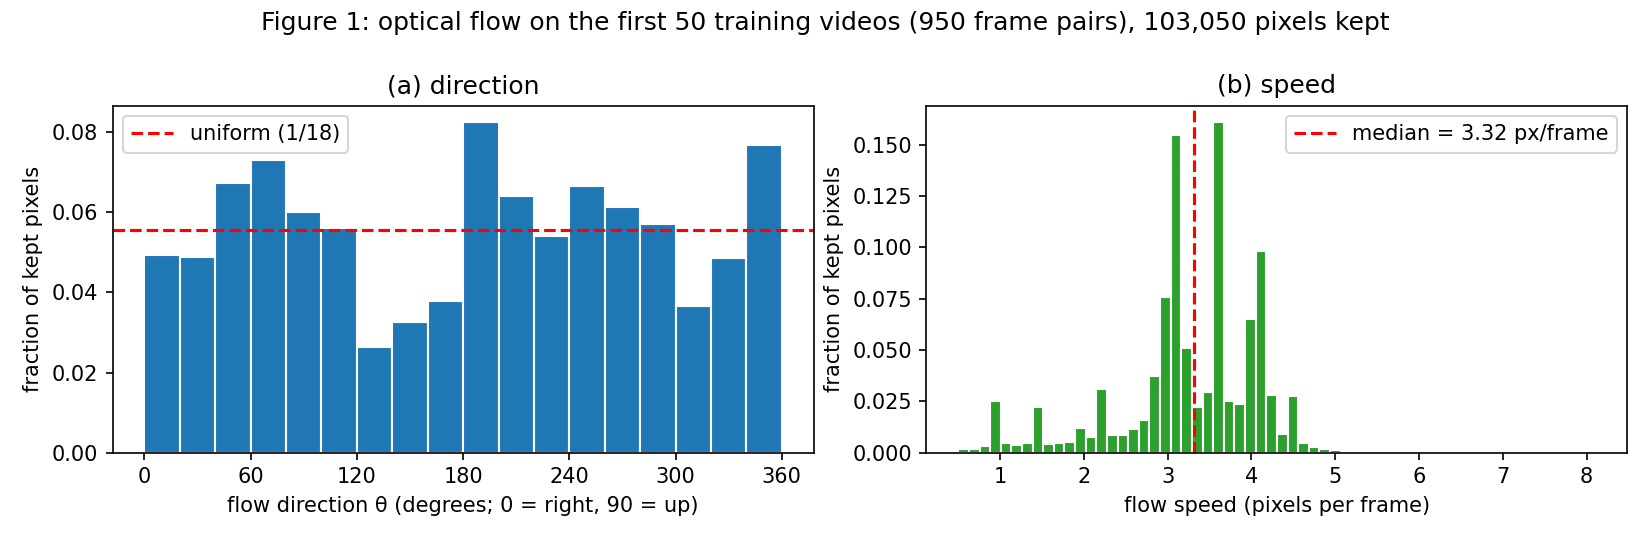
\includegraphics[width=\linewidth]{figures/figure1.png}
\caption{Dense optical flow (Farneback) on the first 50 training videos (950 frame pairs).
(a) Flow direction $\theta=\operatorname{atan2}(-d_y,d_x)$, 18 bins of $20^\circ$; the dashed line is the uniform level $1/18$.
(b) Flow speed in pixels per frame. Median speed \textbf{3.32 px/frame}, \textbf{103,050 pixels kept}. 10th/90th percentiles: 2.14 / 4.12 px/frame.}
\end{figure}

\q{Q2.1}
\textbf{Direction.} Every $20^\circ$ bin of Figure~1(a) contains between 0.026 and 0.083 of the kept pixels, against a uniform level of 0.056. No direction is absent.
\begin{itemize}
  \item Mirroring maps $\theta\mapsto180^\circ-\theta$, and a $90^\circ$ rotation maps $\theta\mapsto\theta+90^\circ$.
  \item Applied to every training video, either would shuffle the bins but produce a histogram of the same broad, roughly uniform shape. The peaks and dips (for example the dip at $120$--$180^\circ$) only move.
  \item So mirrored or rotated \emph{trajectories} are already familiar; what is unfamiliar is the mirrored or rotated \emph{digits}.
\end{itemize}
\textbf{Speed.} A typical speed is about 3.3 px per frame, and nearly all motion is between 2 and 5 px per frame. At $2\times$ this becomes about 6.6 px per model step, and at $3\times$ about 10 px; displacements that large essentially never occur at $1\times$ (the 90th percentile is 4.1).

\textbf{Bias from overlaps.} Where digits overlap, optical flow mixes two motions and is unreliable, so some kept pixels have wrong directions and speeds. This adds noise to both histograms. It cannot remove whole directions, though: digits move in straight lines between bounces, and each of the roughly 100 digits contributes many non-overlapping frames. Speeds above 5 px are absent with or without overlaps. The conclusion is unchanged.

\q{Q2.2}
\begin{itemize}
  \item \textbf{Mirror:} changes the digits' \emph{appearance} (a mirrored 2 is not a 2). It only relabels directions, and given Figure~1(a) it leaves the motion statistics essentially unchanged.
  \item \textbf{Rotation:} also changes \emph{appearance}, more strongly (a rotated 7 resembles no digit). It leaves the motion statistics essentially unchanged, and speed is identical.
  \item \textbf{Speed-up:} changes only the \emph{motion statistics} (2--3$\times$ larger displacement per step); the digits look exactly the same.
\end{itemize}
Each transformation therefore moves the test data along a different axis: appearance only, or motion only. That isolates the cause of a failure, like a controlled experiment that changes one variable at a time.

\subsection*{2. Baseline: ConvLSTM}
\addcontentsline{toc}{subsection}{2. Baseline: ConvLSTM}

\begin{table}[H]
\centering\small
\caption{Test-split errors at $1\times$, $t=1$. MSE$_h$ is the per-horizon pixel MSE; $E^{(5)}$ is their mean.}
\resizebox{\linewidth}{!}{%
\begin{tabular}{@{}l l l l l l l r@{}}
\toprule
Model & MSE$_1$ & MSE$_2$ & MSE$_3$ & MSE$_4$ & MSE$_5$ & $E^{(5)}$ & Params\\
\midrule
A & 0.0172 (0.0174, 0.0169) & 0.0206 (0.021, 0.0202) & 0.0228 (0.0233, 0.0223) & 0.0246 (0.025, 0.0241) & 0.0262 (0.0267, 0.0258) & 0.0223 (0.0227, 0.0219) & 480,784\\
Blank & 0.0426 & 0.0426 & 0.0426 & 0.0425 & 0.0425 & 0.0426 & 0\\
Copy-last & 0.0492 & 0.0604 & 0.0669 & 0.0708 & 0.0732 & 0.0641 & 0\\
\bottomrule
\end{tabular}}
\end{table}

\begin{figure}[H]
\centering
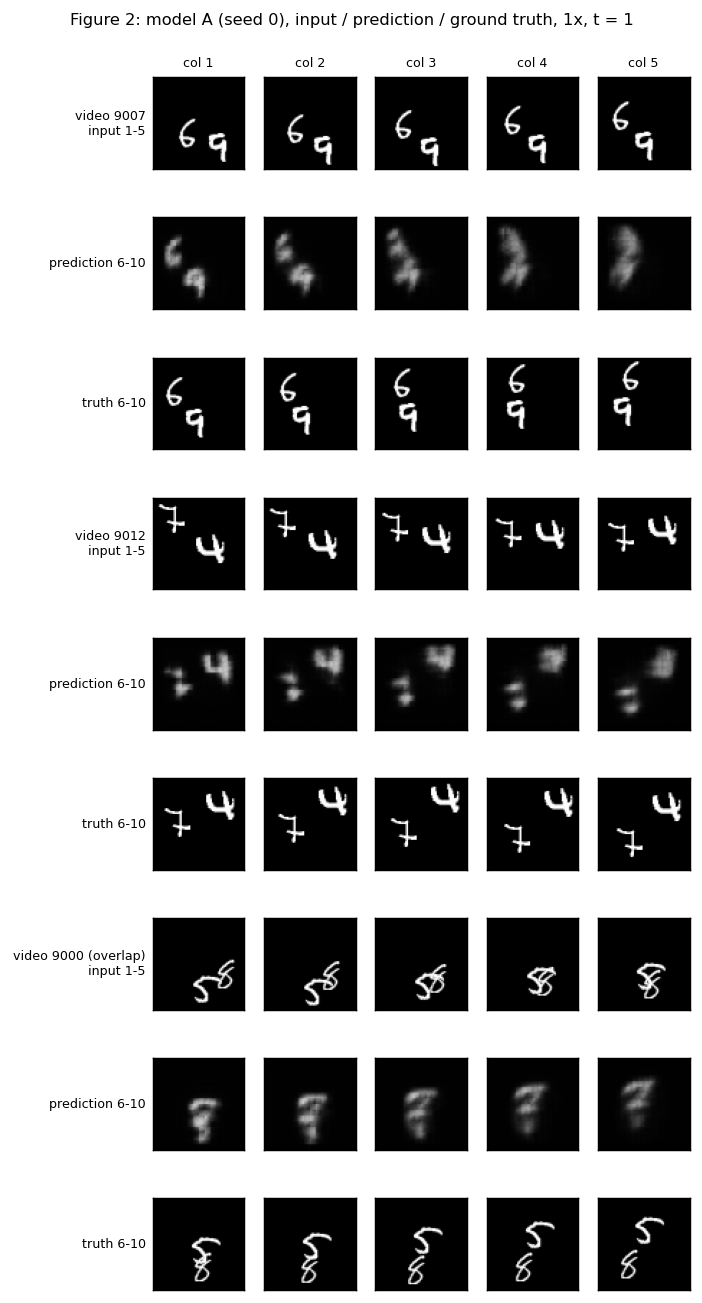
\includegraphics[height=0.62\textheight]{figures/figure2.png}
\caption{Model A (seed 0), $1\times$, $t=1$: input frames 1--5, prediction and ground truth for frames 6--10. Test videos 9007 and 9012 (separate digits) and 9000 (overlapping digits).}
\end{figure}

\q{Q2.3}
\textbf{Model A's reach is 8 original pixels per time step.}

Conventions: a $3\times3$ convolution with stride 1 moves information at most one cell; one cell of the folded $16\times16$ grid is 4 px; $1\times1$ convolutions, \texttt{pixel\_unshuffle} and \texttt{pixel\_shuffle} move nothing. The paths within one step $\tau$:
\begin{itemize}
\item \textbf{New input $u_\tau\to\hat x_{\tau+1}$:} fold (0) $\to$ layer-1 gate convolution on $[u_\tau,h^{(1)}_{\tau-1}]$ (1 cell) $\to$ $h^{(1)}_\tau$ $\to$ layer-2 gate convolution on $[h^{(1)}_\tau,h^{(2)}_{\tau-1}]$ (1 cell) $\to$ $1\times1$ head (0) $\to$ unfold (0). Total \textbf{2 cells}.
\item \textbf{$h^{(1)}_{\tau-1}\to\hat x_{\tau+1}$:} the same two convolutions, \textbf{2 cells}.
\item \textbf{$h^{(2)}_{\tau-1}\to\hat x_{\tau+1}$:} only the layer-2 convolution, \textbf{1 cell}.
\item The cell states $c^{(\ell)}$ are updated element-wise ($\sigma(f)\odot c+\sigma(i)\odot\tanh g$), which adds no spatial movement. Each gate comes from \emph{one} convolution, so gates do not compound within a layer.
\end{itemize}
The longest path is 2 cells $\times$ 4 px = \textbf{8 px}. The $4\times4$ patch width is not added.

\q{Q2.4}
\textbf{Against the reference predictors.} Model A has $E^{(5)}=0.0223$, about half of Blank (0.0426) and about a third of Copy-last (0.0641), so it uses the motion.
\begin{itemize}
  \item Copy-last is \emph{worse} than Blank: a digit drawn where it \emph{was} is wrong twice, once where it no longer is and once where it now is.
  \item Model A beats both at every horizon. Its MSE grows steadily from 0.0172 ($h=1$) to 0.0262 ($h=5$), about $+50\%$.
  \item Figure~2 shows why. The rollout feeds back its own blurred predictions, so errors compound (L5 pp.10--11). Digits are sharp-ish at $h=1$ and become grey blobs by $h=5$, with positions roughly right but shapes lost.
\end{itemize}
\textbf{When digits overlap} (video 9000), the model cannot tell which digit is which. In the truth the 5 separates upwards and the 8 downwards; model A predicts a single blob that stays in place and fades, and never separates the digits. Under a squared-error loss, the best guess between two possible futures is their average, which looks like a smear.

\q{Q2.5} \emph{Prediction before ``Testing the Baseline'':}

No written prediction was committed to the repository before the experiments in ``Testing the Baseline'' were run, so there is no original version to reproduce here. I report this openly rather than reconstruct a prediction after seeing the results; the analysis in Q2.6--Q2.10 is written from the measured results.

\subsection*{3. Testing the Baseline}
\addcontentsline{toc}{subsection}{3. Testing the Baseline}

\begin{table}[H]
\centering\small
\caption{Mirror ($M$) and rotation ($R$): consistency gap $C_T$ and transformed error $E_T$ ($1\times$, $t=1$, test split).}
\resizebox{\linewidth}{!}{%
\begin{tabular}{@{}l l l l l l@{}}
\toprule
Model & $E^{(5)}$ & $C_M$ & $E_M$ & $C_R$ & $E_R$\\
\midrule
A & 0.0223 (0.0227, 0.0219) & 0.00187 (0.00201, 0.00173) & 0.0229 (0.0233, 0.0224) & 0.00317 (0.00348, 0.00285) & 0.0239 (0.0244, 0.0234)\\
Blank & 0.0426 & 0 & 0.0426 & 0 & 0.0426\\
Copy-last & 0.0641 & 0 & 0.0641 & 0 & 0.0641\\
\bottomrule
\end{tabular}}
\end{table}

\begin{figure}[H]
\centering
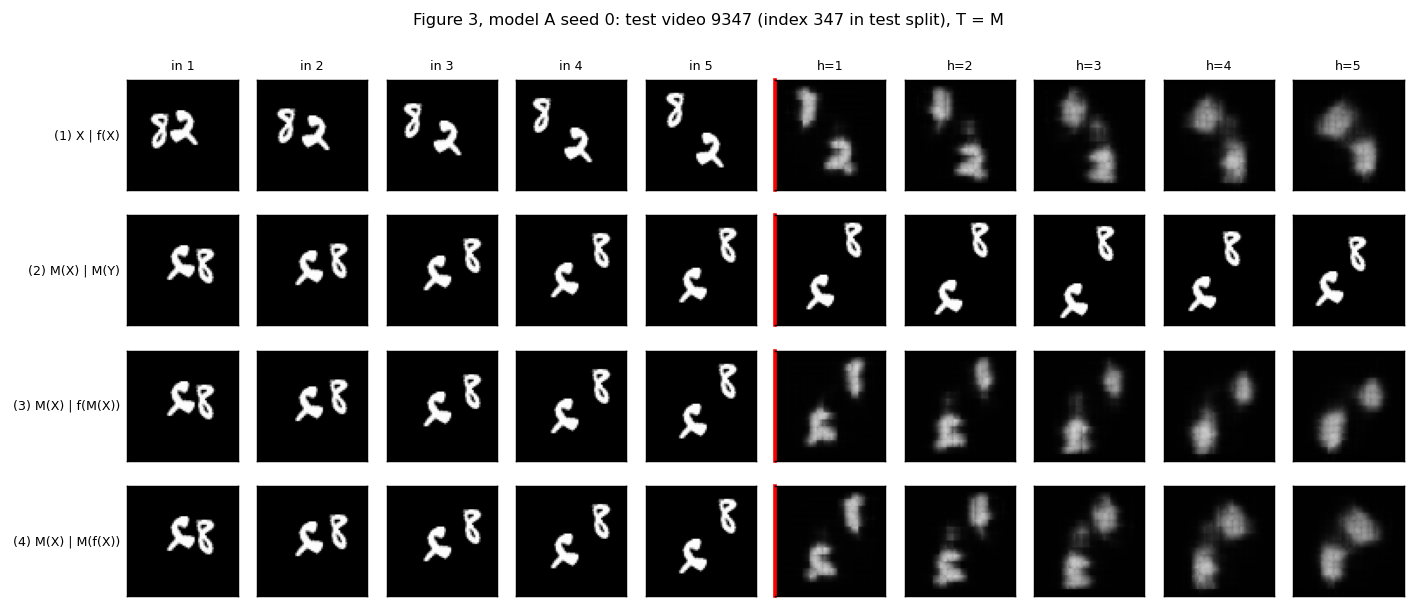
\includegraphics[width=\linewidth]{figures/figure3_M1_video9347.png}\\[2pt]
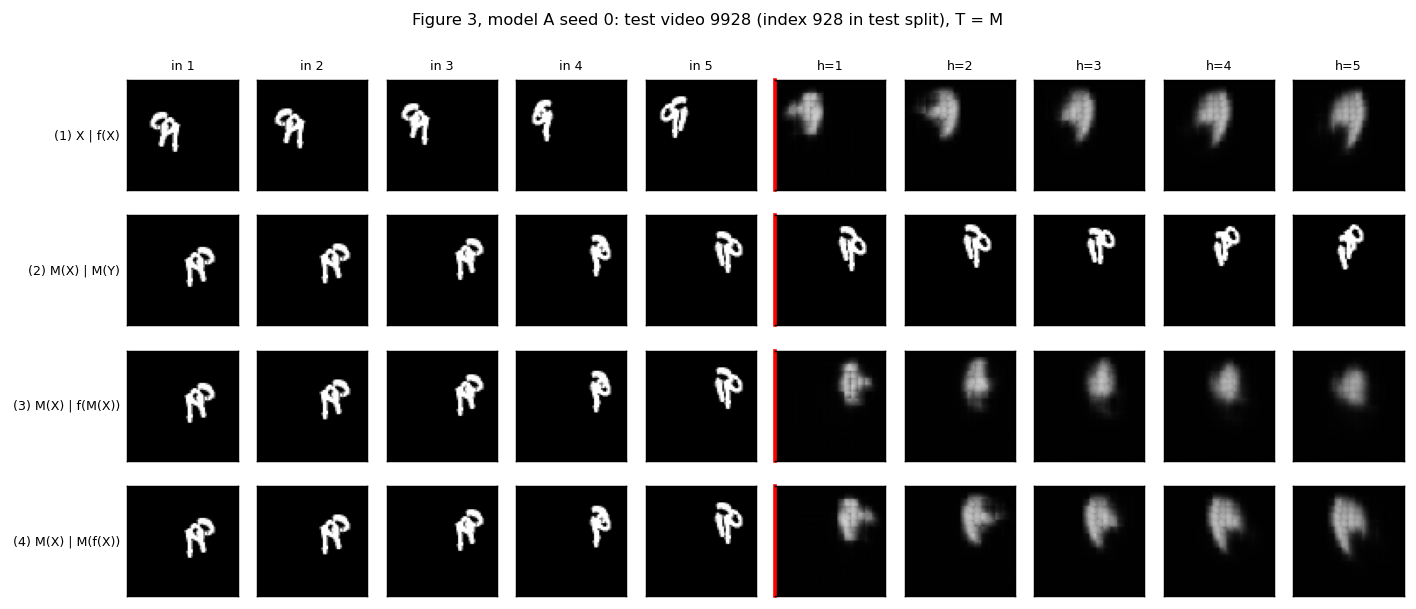
\includegraphics[width=\linewidth]{figures/figure3_M2_video9928.png}
\caption{(Part 1) Seed-0 model A, the two test videos with the largest per-video $C_M$ (9347, 9928). Rows: (1) $X\,|\,f(X)$; (2) $T(X)\,|\,T(Y)$; (3) $T(X)\,|\,f(T(X))$; (4) $T(X)\,|\,T(f(X))$. GIFs:
\gif{Question2/outputs/nb3_test_baseline/gifs/figure3_M1_video9347.gif},
\gif{Question2/outputs/nb3_test_baseline/gifs/figure3_M2_video9928.gif}.}
\end{figure}
\begin{figure}[H]\ContinuedFloat
\centering
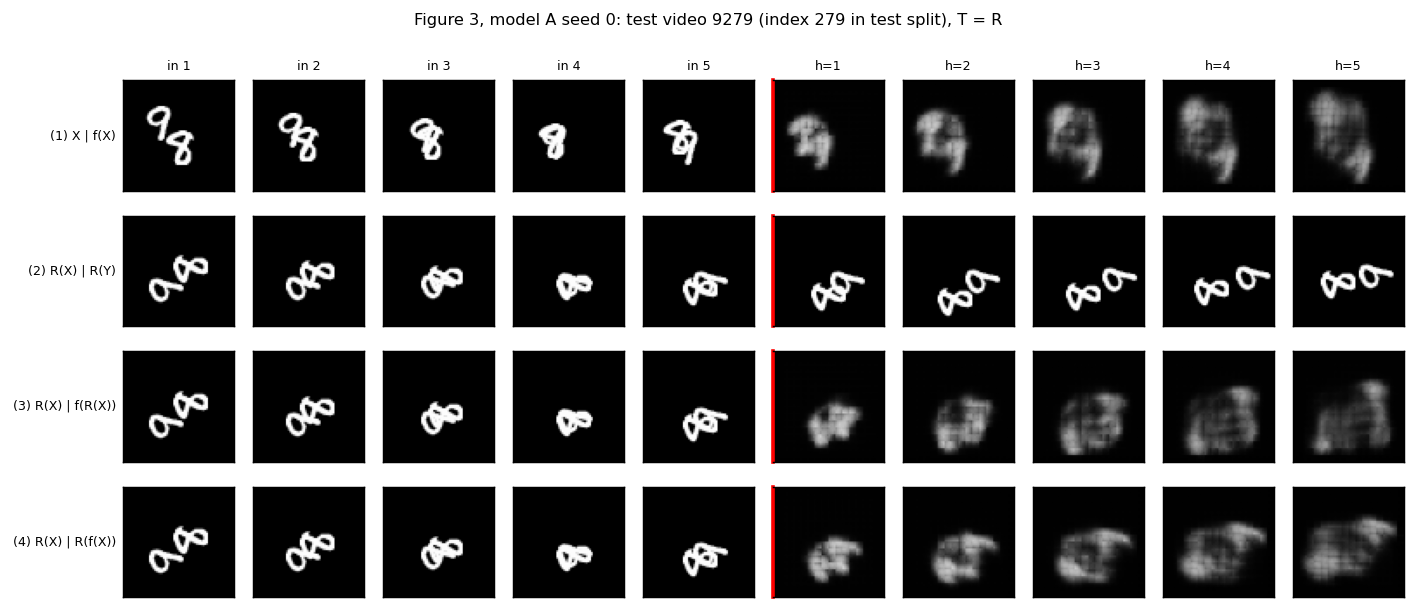
\includegraphics[width=\linewidth]{figures/figure3_R1_video9279.png}\\[2pt]
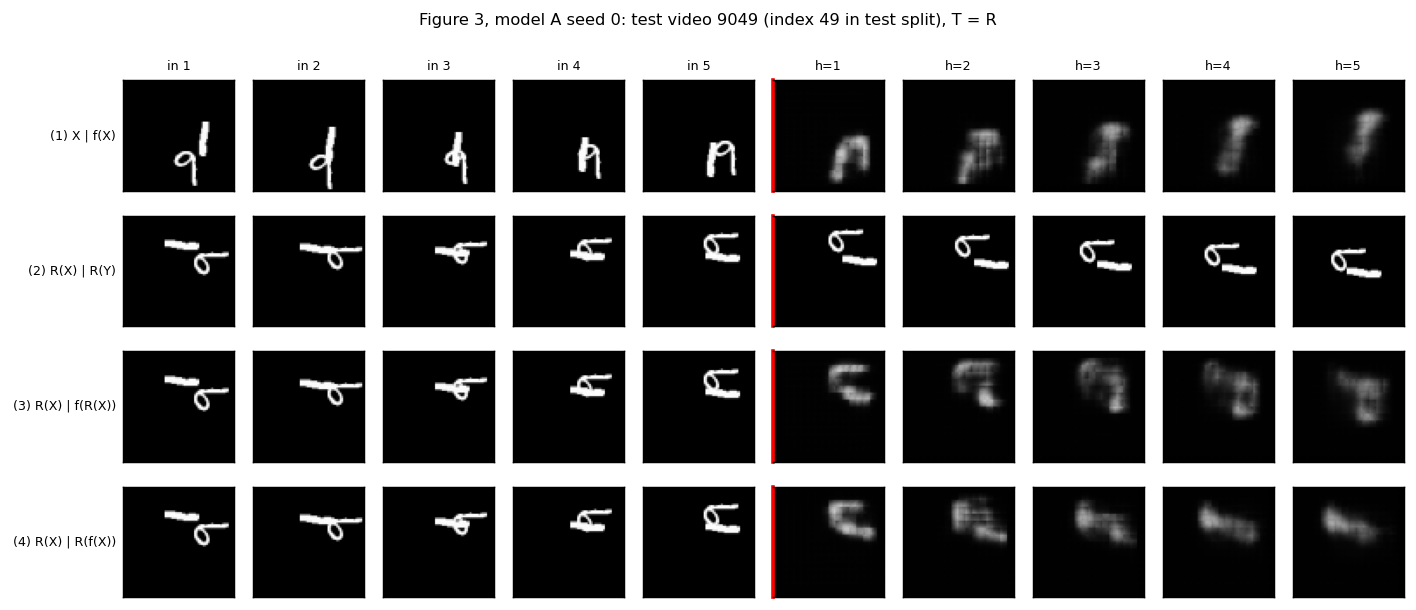
\includegraphics[width=\linewidth]{figures/figure3_R2_video9049.png}
\caption{(Part 2) The two test videos with the largest per-video $C_R$ (9279, 9049); same rows. GIFs:
\gif{Question2/outputs/nb3_test_baseline/gifs/figure3_R1_video9279.gif},
\gif{Question2/outputs/nb3_test_baseline/gifs/figure3_R2_video9049.gif}.}
\end{figure}

\begin{figure}[H]
\centering
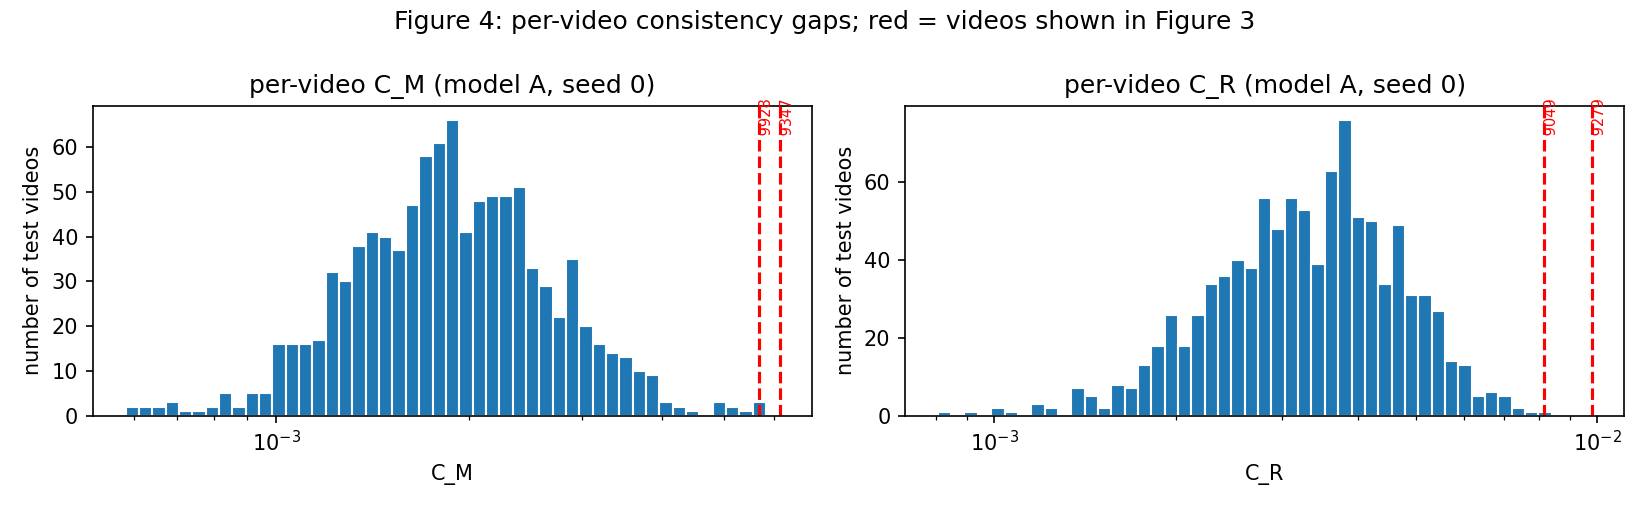
\includegraphics[width=\linewidth]{figures/figure4.png}
\caption{Histograms of per-video $C_M$ and $C_R$ for seed-0 model A over the 1,000 test videos (log scale). Red lines mark the Figure~3 videos.}
\end{figure}

\q{Q2.6}
\begin{itemize}
  \item Blank and Copy-last are exactly consistent because their output is built from the input pixels only, with no notion of motion: mirroring or rotating them commutes trivially. Yet they are the two worst forecasters ($E_M=E_R=0.0426$ and $0.0641$).
  \item A small $C_T$ therefore only says that a model treats the transformed scene \emph{the same way} as the original, not that it treats either one \emph{correctly}. Perfect consistency can be achieved by ignoring the motion altogether.
  \item $E_T$ measures correctness on the transformed scene, so the two must be read together. Low $C_T$ with low $E_T$ is a model that generalises; low $C_T$ with high $E_T$ is a model that is consistently wrong.
\end{itemize}

\q{Q2.7}
\textbf{Video 9279, rotation (Figure~3, part 2, top).}
\begin{itemize}
  \item \emph{Truth (row 2):} two digits (a 9 and an 8) overlap during the input frames and then separate. The 8 moves left and down, and the 9 moves right, with the gap widening at every horizon.
  \item \emph{Row 3}, the model on the rotated video: a single, roughly round blob that grows and drifts up and to the right. The two digits are never separated, both are lost inside one smear by $h=3$, and no digit shape survives.
  \item \emph{Row 4}, the rotated normal prediction: also one blob, but elongated \emph{horizontally}, with mass spreading to the right, which is the direction in which the true 9 leaves. In the original orientation, the model at least ``knows'' the digits are pulling apart along that axis.
\end{itemize}
So on the rotated input the model's account of the motion changes from \emph{two digits separating along one axis, blurred} to \emph{one merged blob drifting the wrong way}.

\q{Q2.8}
\begin{itemize}
  \item \textbf{Rotation is harder for model A.} Its gap is 70\% larger ($C_R=0.00317$ vs $C_M=0.00187$). The transformed error rises more: $E_R=0.0239$ vs $E_M=0.0229$, against $E^{(5)}=0.0223$ on the original videos. Figure~4 shows the whole $C_R$ distribution sitting to the right of $C_M$, so this is not a few outliers.
  \item \textbf{The motion is not the cause.} From Q2.1, rotated and mirrored trajectories are equally familiar: every direction already occurs in training at a similar rate, and speeds are unchanged.
  \item \textbf{Appearance is the cause.} From Q2.2, the only thing that differs between the two tests is how much they change the digits. A mirror leaves several digits nearly unchanged (0, 1, 8) and others still digit-like. A $90^\circ$ rotation turns every digit into a shape never seen in training.
  \item So model A's motion rule is partly tied to what the digits look like. Model B confirms this (Q2.13).
\end{itemize}

\begin{table}[H]
\centering\small
\caption{Faster motion (test split, $t=1$). $E^{(2)}$ uses the first two horizons only.}
\resizebox{\linewidth}{!}{%
\begin{tabular}{@{}l l l l l l@{}}
\toprule
Model & $E^{(2)}$ $1\times$ & $E^{(2)}$ $2\times$ & $E^{(2)}$ $3\times$ & $E^{(5)}$ $1\times$ & $E^{(5)}$ $2\times$\\
\midrule
A & 0.0189 (0.0192, 0.0185) & 0.045 (0.0454, 0.0445) & 0.0527 (0.0535, 0.0518) & 0.0223 (0.0227, 0.0219) & 0.0498 (0.0505, 0.049)\\
Copy-last & 0.0548 & 0.0661 & 0.0703 & 0.0641 & 0.0719\\
\bottomrule
\end{tabular}}
\end{table}

\begin{figure}[H]
\centering
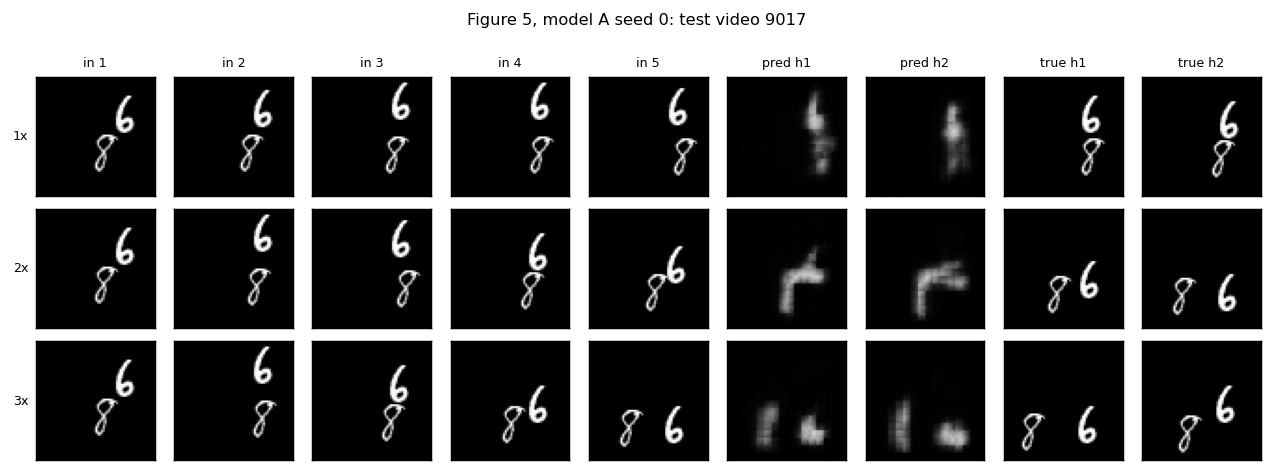
\includegraphics[width=\linewidth]{figures/figure5.png}
\caption{Seed-0 model A on test video 9017 (no overlap in the displayed true frames) at $1\times$, $2\times$, $3\times$: five inputs, the first two predicted frames and the first two true frames.}
\end{figure}

\q{Q2.9}
\textbf{Model A falls apart at $2\times$.}
\begin{itemize}
  \item $E^{(2)}$ goes from 0.0189 to 0.045 ($2.4\times$), and to 0.0527 at $3\times$, approaching Copy-last (0.0661 / 0.0703).
  \item This \emph{disagrees} with the reach estimate. At $2\times$ the median displacement is about 6.6 px, inside the 8 px reach; only $3\times$ (about 10 px) exceeds it.
\end{itemize}
\textbf{What the estimate missed:}
\begin{itemize}
  \item reach is an upper bound on what the architecture \emph{can} connect, not what the weights \emph{do}; a model trained only on 3--4 px jumps has no reason to use its full 8 px reach;
  \item $2\times$ motion is completely absent from training (Figure~1b), so the failure there is about unfamiliar motion, not reach;
  \item the reach applies per recurrent step, but tracking needs the matching to happen reliably at every step of the rollout.
\end{itemize}
\textbf{What the failure looks like} (Figure~5):
\begin{itemize}
  \item \emph{1$\times$:} both digits are kept near their true positions, slightly blurred.
  \item \emph{2$\times$:} the 6 and the 8 merge into one L-shaped smear between their old and new positions. The digits \emph{stall} and lag behind, and their shapes \emph{blur} together. The model is partly continuing the old motion at its familiar slow speed and averaging over where the digits might be.
  \item \emph{3$\times$:} two faint, shapeless blobs at roughly plausible places. The digits nearly \emph{vanish}: unable to link the new positions to the stored ones, the model hedges towards the mean (dark) frame, which squared error rewards.
\end{itemize}

\q{Q2.10}
\textbf{No.} Model A has never seen fast motion \emph{and} has a reach of only 8 px, so both explanations predict a failure at $3\times$. Its results alone cannot separate them.

\textbf{Proposed experiment:} vary one factor at a time.
\begin{itemize}
  \item \textbf{Change the data only:} retrain the same architecture with speed augmentation (model C).
  \item \textbf{Change the architecture only:} enlarge the reach while keeping the data (model D, compared with C).
\end{itemize}
How to read the outcome:
\begin{itemize}
  \item If C fixes a speed, that failure was \emph{unfamiliar motion}.
  \item If C still fails at $3\times$ but D (same data, larger reach) succeeds, the remaining failure is \emph{architectural reach}.
  \item A complementary check: a larger-reach model trained at $1\times$ only. If it still fails at $2\times$, the problem is familiarity, not reach.
\end{itemize}

\subsection*{4. What Can Data Fix?}
\addcontentsline{toc}{subsection}{4. What Can Data Fix?}

\q{Q2.11} \emph{Prediction before training models B--D:}

No written prediction was committed before models B--D were trained, so there is no original version to reproduce here. As with Q2.5, I state this openly instead of writing a prediction with hindsight; Q2.12--Q2.14 are based on the measured results.

\begin{table}[H]
\centering\scriptsize
\setlength{\tabcolsep}{3pt}
\caption{Models A--D on the test split ($t=1$). Training time is the mean wall-clock seconds per epoch over 30 epochs. Inference is the seconds to predict the 1,000 original test videos at batch 32. Hardware: Tesla T4.}
\resizebox{\linewidth}{!}{%
\begin{tabular}{@{}l l l l l l l l l r r r@{}}
\toprule
Model & $E^{(5)}$ $1\times$ & $C_M$ & $E_M$ & $C_R$ & $E_R$ & $E^{(2)}$ $1\times$ & $E^{(2)}$ $2\times$ & $E^{(2)}$ $3\times$ & Params & Train s/ep. & Infer.\ s\\
\midrule
A & 0.0223 (0.0227, 0.0219) & 0.00187 (0.00201, 0.00173) & 0.0229 (0.0233, 0.0224) & 0.00317 (0.00348, 0.00285) & 0.0239 (0.0244, 0.0234) & 0.0189 (0.0192, 0.0185) & 0.045 (0.0454, 0.0445) & 0.0527 (0.0535, 0.0518) & 480,784 & 10.7 & 0.414\\
B & 0.0223 (0.0225, 0.0221) & 0.0016 (0.00146, 0.00175) & 0.0223 (0.0225, 0.0221) & 0.00168 (0.00161, 0.00175) & 0.0222 (0.0224, 0.0219) & 0.0186 (0.0186, 0.0185) & 0.0446 (0.0455, 0.0437) & 0.0511 (0.053, 0.0491) & 480,784 & 12.1 & 0.414\\
C & 0.0267 (0.0272, 0.0263) & 0.00135 (0.00117, 0.00154) & 0.0269 (0.0273, 0.0265) & 0.00258 (0.0022, 0.00295) & 0.0279 (0.0282, 0.0276) & 0.0232 (0.0237, 0.0227) & 0.0288 (0.0292, 0.0285) & 0.0333 (0.0335, 0.0331) & 480,784 & 11.7 & 0.413\\
D & 0.0212 (0.0212, 0.0212) & 0.00267 (0.00273, 0.0026) & 0.0221 (0.022, 0.0221) & 0.00423 (0.00425, 0.00422) & 0.0235 (0.0235, 0.0235) & 0.0184 (0.0184, 0.0184) & 0.0224 (0.0224, 0.0225) & 0.026 (0.0259, 0.026) & 595,520 & 6.35 & 0.252\\
\bottomrule
\end{tabular}}
\end{table}
\noindent{\footnotesize Per-seed timings: A 10.7 (10.7, 10.7) / 0.414 (0.416, 0.413); B 12.1 (12.2, 12.1) / 0.414 (0.415, 0.413); C 11.7 (11.6, 11.7) / 0.413 (0.413, 0.413); D 6.35 (6.4, 6.29) / 0.252 (0.251, 0.253).}

\q{Q2.12}
\textbf{Model D (\texttt{D\_p8\_ln}).} A ConvLSTM with the same two layers, 64 hidden channels, $3\times3$ kernels, $1\times1$ head, sigmoid output, 9-step rollout and training protocol as A, with two changes:
\begin{itemize}
  \item \textbf{$8\times8$ folding:} \texttt{pixel\_unshuffle}($\cdot$, 8), so a $1\times64\times64$ frame becomes $64\times8\times8$. The head maps 64 to 64 channels before \texttt{pixel\_shuffle}($\cdot$, 8).
  \item \textbf{Per-pixel gate normalisation:} the pre-activations of each gate are normalised over channels \emph{at each spatial position separately}, with a learned gain and shift (1,024 parameters).
\end{itemize}
In total D has \textbf{595,520} parameters, within the limit of 721,176.

\textbf{Reach}, by the same paths as Q2.3:
\begin{itemize}
  \item the longest path is still new input (or $h^{(1)}_{\tau-1}$) $\to$ layer-1 $3\times3$ convolution $\to$ layer-2 $3\times3$ convolution, which is 2 cells;
  \item one cell is now \textbf{8 px};
  \item the normalisation pools over channels only, never over space, so it adds no spatial path.
\end{itemize}
Reach $=2\times8=$ \textbf{16 px per step}, strictly larger than A's 8 px and above the roughly 10 px median displacement at $3\times$.

\textbf{How D was chosen} (validation split and training loss only; never the test split):
\begin{itemize}
  \item \emph{$5\times5$ kernels} (46 channels, 709,520 parameters, reach 16 px): collapsed on seed 0. From epoch 2 the training loss stayed at 0.0402, the loss of predicting one constant average frame.
  \item \emph{$8\times8$ folding without normalisation} (chosen over dilated $3\times3$ kernels on validation $E^{(2)}$ after 8 epochs): collapsed the same way on seed 0.
  \item In both cases seed 1 trained, and model C on the same data never collapsed.
  \item The wider-reach networks got stuck at the ``mean frame'' solution under the fixed optimiser (saturated gates give vanishing gradients). Per-pixel gate normalisation keeps the gate inputs in the sigmoid's sensitive range without changing reach. With it, both seeds trained (final training loss 0.0231 / 0.0234).
\end{itemize}

\q{Q2.13}
\textbf{Mirror and rotation failures: appearance.}
\begin{itemize}
  \item B changes only the digits' appearance in training (symmetry augmentation). It roughly halves the rotation gap ($C_R$ 0.00317 $\to$ 0.00168) and brings $E_M=0.0223$ and $E_R=0.0222$ down to its own $E^{(5)}=0.0223$: B is as good on transformed videos as on originals.
  \item Its speed errors are unchanged (0.0446 / 0.0511), so B fixed exactly the appearance axis.
  \item C and D, which add no transformed digits, do not reduce $C_R$ (0.00258, 0.00423).
\end{itemize}
\textbf{$2\times$ failure: unfamiliar motion.}
\begin{itemize}
  \item With the same architecture and reach, C cuts $E^{(2)}$ at $2\times$ from 0.045 to 0.0288.
  \item $2\times$ (about 6.6 px) is inside A's 8 px reach, so data alone could fix it.
\end{itemize}
\textbf{$3\times$ failure: unfamiliar motion and architectural reach.}
\begin{itemize}
  \item C improves $3\times$ (0.0527 $\to$ 0.0333), but it remains C's worst speed. D, trained on the same speed-augmented data with twice the reach, reaches 0.026.
  \item Caveat: D is also better at $1\times$ (0.0184 vs C's 0.0232), so part of its gain is general rather than reach-specific. Still, its $3\times$/$1\times$ ratio (1.41) is similar to C's (1.44) while all of D's errors are lower.
\end{itemize}
\textbf{Why more data cannot carry information further than the architecture allows.} Training data changes the \emph{weights}, but reach is fixed by the \emph{wiring}: the number of spatial convolutions per step times their span and the patch size. If a digit jumps 10 px and the network connects at most 8 px per step, then no setting of the weights links its stored old position to its new position within one update. More examples of fast motion only teach the model to hedge more cleverly.

\q{Q2.14}
\begin{itemize}
  \item \textbf{B:} cost nothing at $1\times$ ($E^{(5)}$ 0.0223 vs 0.0223) and gained consistency. Clearly worth it.
  \item \textbf{C:} \emph{did} cost $1\times$ accuracy, $E^{(5)}$ 0.0223 $\to$ 0.0267 (+20\%). Its capacity is now shared across three speeds and only a third of its training windows are $1\times$. In return, $2\times$ and $3\times$ errors fell by 36--37\%, so it is worth it whenever the speed at test time is unknown.
  \item \textbf{D:} cost nothing at $1\times$ and is the best model there ($E^{(5)}=0.0212$). It is also faster: 6.35 s per epoch and 0.252 s inference, against 10.7 s and 0.414 s for A, because the $8\times8$ grid has 4 times fewer cells.
  \item \textbf{But D gave up consistency:} $C_R=0.00423$, the worst of A--D. The final model addresses that.
\end{itemize}

\subsection*{5. The Final Model}
\addcontentsline{toc}{subsection}{5. The Final Model}

\noindent\textbf{Why $\bar f$ is exactly consistent.} Let $h\in G$. Then
\[ \bar f(hX)=\tfrac18\sum_{g\in G} g^{-1}f(ghX). \]
Substitute $g'=gh$. As $g$ runs over $G$, so does $g'$, because right-multiplication by $h$ is a bijection of the group. Since $g^{-1}=h\,g'^{-1}$:
\[ \bar f(hX)=\tfrac18\sum_{g'\in G} h\,g'^{-1}f(g'X)=h\,\bar f(X), \]
using the fact that $h$ is linear (it permutes pixels), so it commutes with averaging. $M$ and $R$ are both in $G$, so $C_M=C_R=0$ for \emph{any} $f$. The measured values (about $10^{-17}$) are floating-point rounding.

\noindent\textbf{Final model:} symmetrised D. Table~5 shows that D is the most accurate at every speed; its only weakness is consistency, which symmetrisation removes exactly. Symmetry augmentation (D+B) is therefore unnecessary for consistency, and was not trained for lack of time.

\begin{table}[H]
\centering\scriptsize
\setlength{\tabcolsep}{3pt}
\caption{Symmetrised forecasters (test split). Training time is that of the underlying learned model; inference includes all 8 transformations, forward passes, inverse transformations and the averaging (Tesla T4).}
\resizebox{\linewidth}{!}{%
\begin{tabular}{@{}l l l l l l l l l r r r@{}}
\toprule
Model & $E^{(5)}$ $1\times$ & $C_M$ & $E_M$ & $C_R$ & $E_R$ & $E^{(2)}$ $1\times$ & $E^{(2)}$ $2\times$ & $E^{(2)}$ $3\times$ & Params & Train s/ep. & Infer.\ s\\
\midrule
sym.\ B & 0.0216 (0.0218, 0.0213) & 8.75e-17 (9.10e-17, 8.40e-17) & 0.0216 (0.0218, 0.0213) & 7.05e-17 (7.31e-17, 6.79e-17) & 0.0216 (0.0218, 0.0213) & 0.0181 (0.0181, 0.018) & 0.0437 (0.0447, 0.0427) & 0.05 (0.0521, 0.048) & 480,784 & 12.1 & 3.3\\
sym.\ D (final) & 0.0209 (0.0209, 0.021) & 8.40e-17 (8.59e-17, 8.20e-17) & 0.0209 (0.0209, 0.021) & 6.77e-17 (6.93e-17, 6.62e-17) & 0.0209 (0.0209, 0.021) & 0.0183 (0.0183, 0.0183) & 0.0222 (0.0221, 0.0222) & 0.0255 (0.0255, 0.0256) & 595,520 & 6.35 & 2.06\\
\bottomrule
\end{tabular}}
\end{table}
\noindent{\footnotesize Per-seed inference: sym.\ B 3.3 (3.26, 3.33) s; sym.\ D 2.06 (2.07, 2.06) s.}

\begin{figure}[H]
\centering
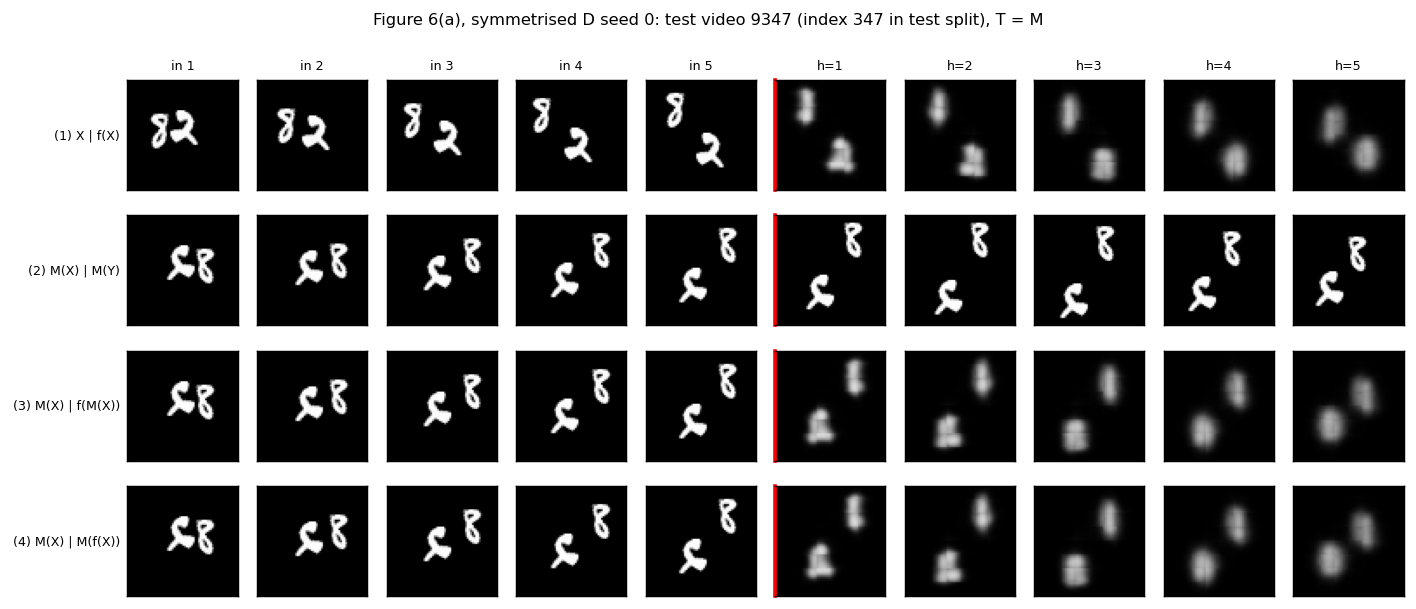
\includegraphics[width=0.93\linewidth]{figures/figure6a_M1_video9347.png}\\[1pt]
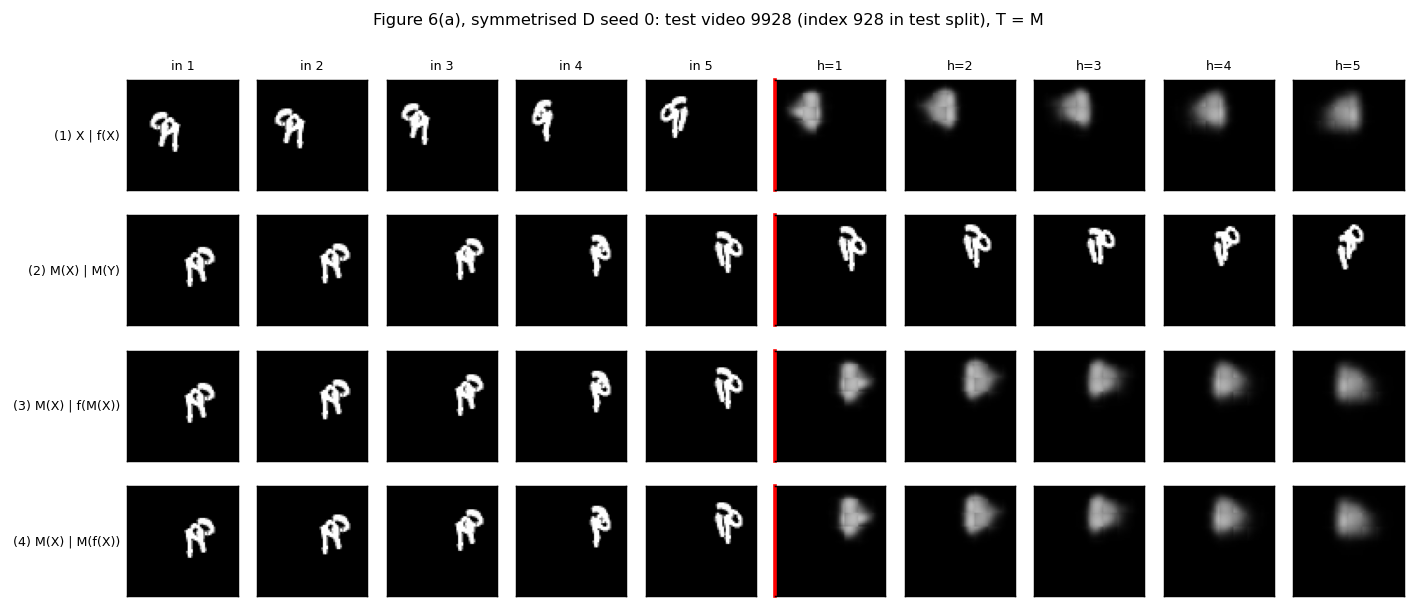
\includegraphics[width=0.93\linewidth]{figures/figure6a_M2_video9928.png}
\caption{(a, part 1) Figure~3 repeated with the final model (symmetrised D, seed 0) on the same videos. GIFs:
\gif{Question2/outputs/nb5_final_model/gifs/figure6a_M1_video9347.gif},
\gif{Question2/outputs/nb5_final_model/gifs/figure6a_M2_video9928.gif}.}
\end{figure}
\begin{figure}[H]\ContinuedFloat
\centering
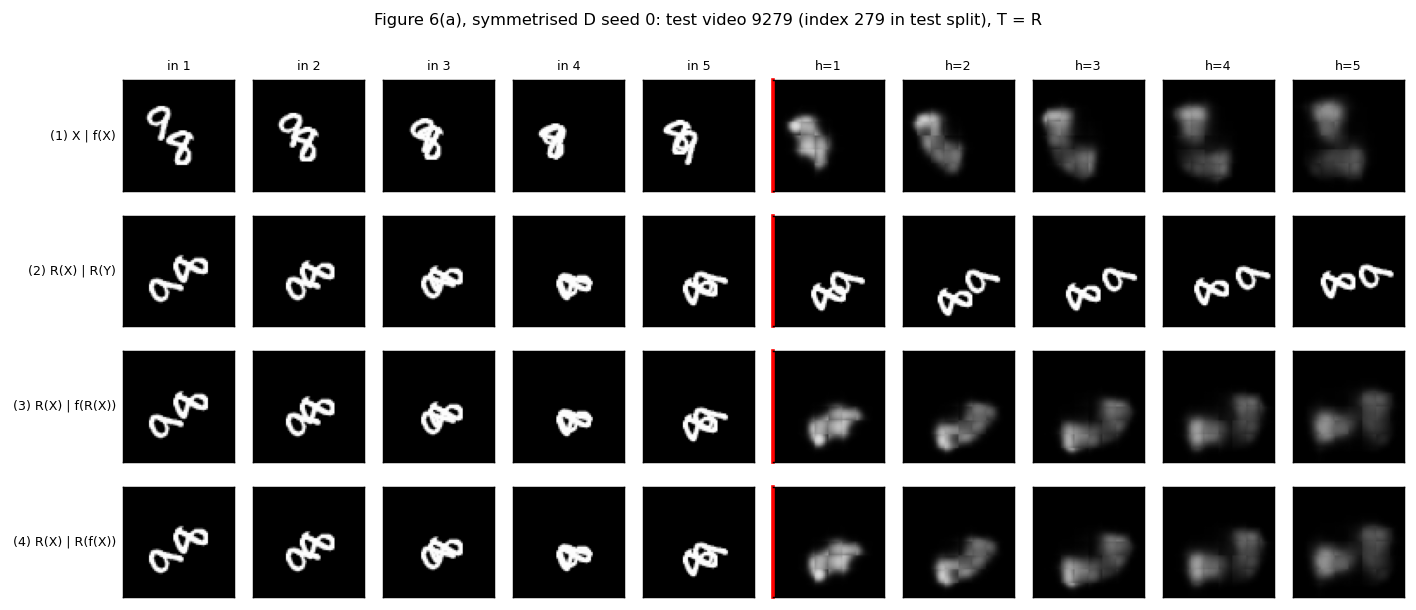
\includegraphics[width=0.93\linewidth]{figures/figure6a_R1_video9279.png}\\[1pt]
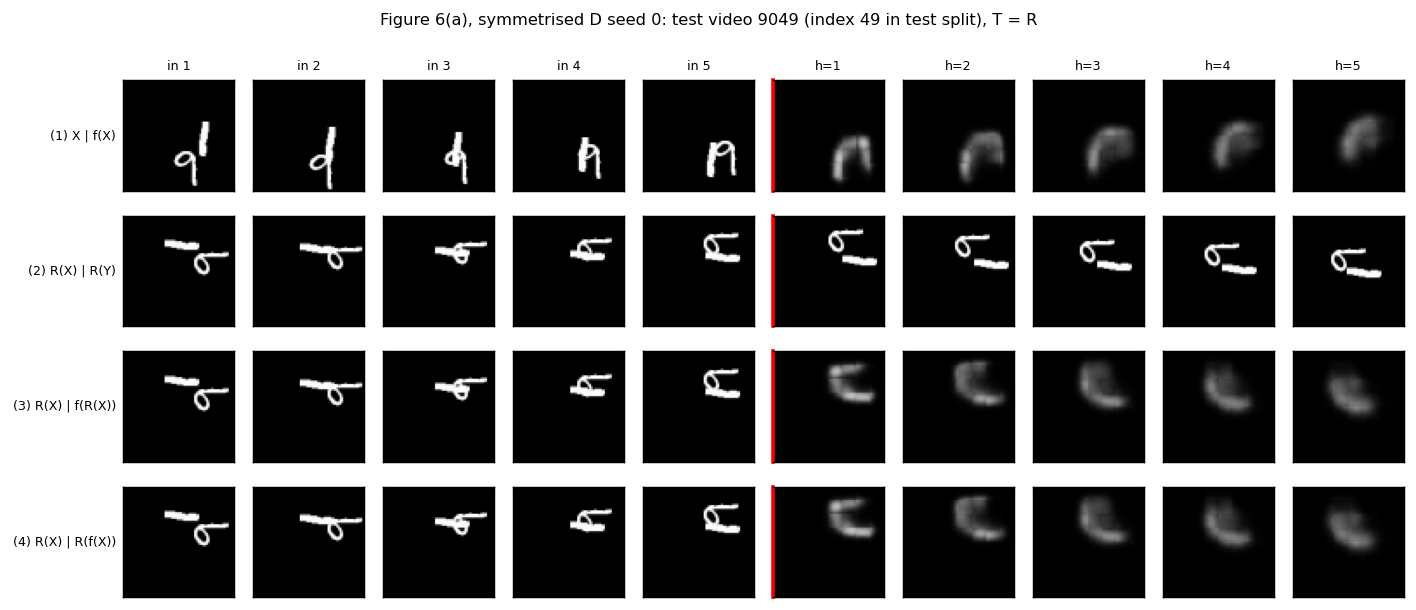
\includegraphics[width=0.93\linewidth]{figures/figure6a_R2_video9049.png}\\[1pt]
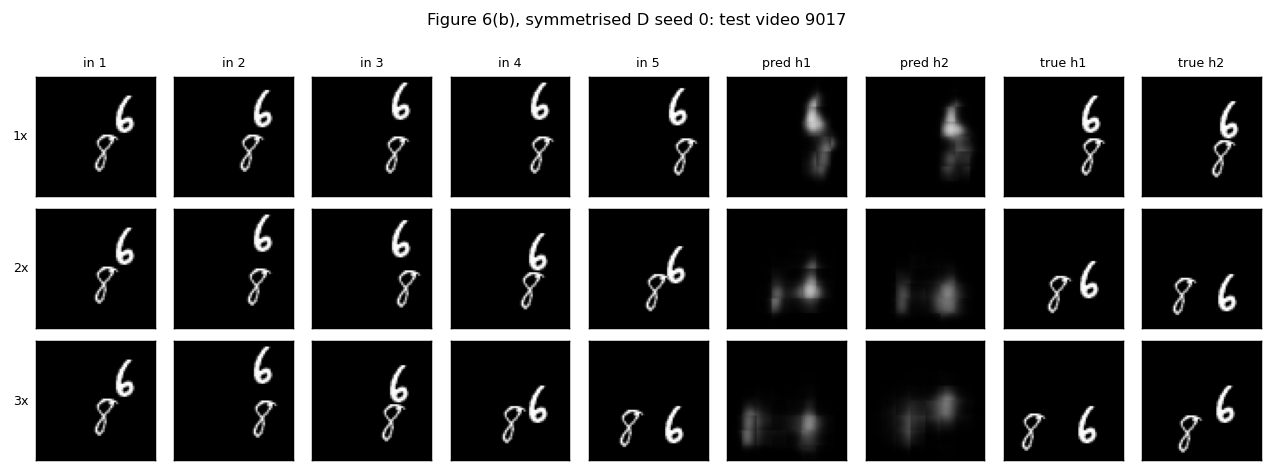
\includegraphics[width=0.93\linewidth]{figures/figure6b.png}
\caption{(a, part 2) The rotation videos with the final model. GIFs:
\gif{Question2/outputs/nb5_final_model/gifs/figure6a_R1_video9279.gif},
\gif{Question2/outputs/nb5_final_model/gifs/figure6a_R2_video9049.gif}.
(b, bottom) Figure~5 repeated with the final model on the same video 9017.}
\end{figure}

\q{Q2.15}
\textbf{Consistency.}
\begin{itemize}
  \item Learned symmetry (B) only \emph{reduces} the gaps ($C_M=0.0016$, $C_R=0.00168$): augmentation shows the model transformed examples, but nothing forces its function to commute with $G$.
  \item Built-in symmetry is \emph{exact} ($\approx10^{-16}$--$10^{-17}$) for any underlying model, by the reindexing argument above. Only it is exact.
\end{itemize}
\textbf{Accuracy.} Symmetrisation slightly \emph{improves} accuracy on the original clips (B: 0.0223 $\to$ 0.0216; D: 0.0212 $\to$ 0.0209). For a model that is not already consistent, $E_M$ and $E_R$ then become identical to $E^{(5)}$: symmetrised D goes from $E_R$ 0.0235 to 0.0209.

\textbf{Inference cost.} About $8\times$ (B: 0.414 s $\to$ 3.3 s; D: 0.252 s $\to$ 2.06 s). Training cost is unchanged.

\textbf{When averaging hurts.} Averaging eight predictions blurs them wherever the eight orientations disagree. It should hurt accuracy when the underlying model is \emph{confidently right} in its familiar orientation but wrong in the others, so that seven bad votes dilute one good one; that happens for a model trained without augmentation and tested on clips where it is reliable.
\begin{itemize}
  \item Here it did \emph{not} hurt MSE. Our base models' predictions are already blurry, and MSE rewards averaging.
  \item It did hurt sharpness visually: the digits in Figure~6 are softer blobs than model A's at $h=1$. A sharpness-sensitive metric (for example SSIM, the structural similarity index) would likely show this cost.
\end{itemize}

\q{Q2.16}
\textbf{Mostly yes, in position; not in shape.} On video 9279 (rotation), Figure~6(a):
\begin{itemize}
  \item rows 3 and 4 are now identical, as guaranteed;
  \item the prediction shows \emph{two} separate blobs, one moving left and down (the 8) and one moving right (the 9), with the gap widening over the horizons as in the truth (row 2). Model A instead merged them into a single drifting smear;
  \item the digits are still not recognisable.
\end{itemize}
\textbf{Which change fixed which part:}
\begin{itemize}
  \item \textbf{Symmetrisation} fixed the inconsistency (rows 3 and 4 agree), and made the rotated video as easy as the original.
  \item \textbf{Model D's architecture and speed-augmented training} fixed the tracking: the digits separate and move in the right directions. Symmetrised B (appearance augmentation, A's 8 px reach) improves consistency but not the speed failures in Table~6.
  \item The remaining failure, blurred shapes, is not fixed by any change. It comes from the squared-error loss and the uncertainty about overlapping digits.
\end{itemize}

\q{Q2.17}
\textbf{Final verdict.} Mostly, yes. The final model has learned \emph{where things move}, not only what training videos look like.
\begin{itemize}
  \item It is exactly consistent under all eight symmetries.
  \item It is equally accurate on mirrored and rotated clips ($E_M=E_R=E^{(5)}=0.0209$).
  \item It degrades gracefully with speed (0.0183 / 0.0222 / 0.0255 at $1\times$/$2\times$/$3\times$, against model A's 0.0189 / 0.045 / 0.0527).
\end{itemize}
A skeptic should be convinced by speeds and orientations held out from training behaving like the training distribution, and by the controlled comparison: A, B, C and D each fix exactly the failure their single change targets.

It has \emph{not} learned \emph{what} moves. Digits blur into shapeless blobs within two or three frames, and overlaps are averaged rather than resolved.

\textbf{One test it has not passed:} motion outside the training speeds, such as $4\times$ (about 13 px per step), where the model has neither the familiarity nor much reach margin.

\newpage
% =====================================================================================
\section*{Use of Generative AI}
\addcontentsline{toc}{section}{Use of Generative AI}
% =====================================================================================

As required by the course AI policy, the prompts, outputs and my edits are listed below. Tool: Claude (Anthropic), used in a coding assistant inside VS Code.

\begin{enumerate}
\item \textbf{Prompt (summary):} ``Explain the concepts required to solve the assignment, with references from the lectures, in simple terms, without abbreviations and without code.''\\
\textbf{Output:} a concept guide (convolution, receptive field, LSTM and ConvLSTM, rollout and teacher forcing, MSE vs MAE, reach, equivariance, symmetrisation, optical flow, space--time composition), with lecture page references, and a section-by-section walkthrough of Q1 and Q2.\\
\textbf{My use/edits:} used as study material to understand the concepts needed for both questions before starting the implementation.

\item \textbf{Prompt:} ``Start the solution of implementation and provide files to run on Kaggle, with comments explaining each cell and lecture references.''\\
\textbf{Output:} \texttt{q2lib.py} and five Kaggle notebooks (data split, transformations, windows, ConvLSTM, training loop, metrics, figures, symmetrised forecaster).\\
\textbf{My use/edits:} ran all five notebooks on Kaggle (Tesla T4 GPU), attached each notebook's output to the next, and returned the outputs and error messages for checking.

\item \textbf{Prompts:} error reports while running the notebooks (missing \texttt{d\_choice.json}, missing \texttt{B\_s0.pt}) and ``is Question 2 complete?''\\
\textbf{Output:} fixes to the checkpoint loading. Diagnosis that model D collapsed on seed 0 (loss stuck at 0.0402) for two designs, and the proposed fix (per-pixel gate normalisation, design \texttt{D\_p8\_ln}).\\
\textbf{My use/edits:} re-ran Notebooks 4 and 5 after each fix and confirmed that both seeds of the final model D trained (final training losses 0.0231 and 0.0234) and that Table~5 and Table~6 were regenerated from the new checkpoints.

\item \textbf{Prompt:} ``Create the report as per requirements (LaTeX).''\\
\textbf{Output:} this LaTeX report: Q1 design proposal draft, Q2 tables from my result files, and draft answers to Q2.1--Q2.17 based on my results and figures.\\
\textbf{My use/edits:} supplied all result files (tables, figures, GIFs, notebook outputs) from which the numbers and figure descriptions were taken, compiled the report on Overleaf and reported the compilation errors, which were then fixed.
\end{enumerate}

\end{document}
